\documentclass[10pt,a4paper]{article}
\usepackage{mathcomp,amssymb,mathptm,theme}
\usepackage[utf8]{inputenc}
\usepackage[francais]{babel}
\usepackage[T1]{fontenc}
\usepackage{amsmath}
\usepackage{amsfonts}
\usepackage{amssymb}
\usepackage{graphicx}
\usepackage{color}
\usepackage{caption}
\usepackage{tikz}
\usepackage{pifont}
\newtheorem{definition}{Definition}[section]
\newtheorem{theorem}{Theroem}[section]
\newcommand{\cmark}{\ding{51}}%
\newcommand{\xmark}{\ding{55}}%
\renewcommand{\thesection}{\arabic{section}}
\newcommand{\rouge}[1]{{\color{red}#1}}
\newcommand{\VERT}[1]{{\color{green}#1}}
\newcommand{\bleu}[1]{\textcolor{black}{$#1$}}
\newcommand{\bl}[1]{\textcolor{black}{#1}}
\newcommand{\Ra}{\ensuremath{\Rightarrow}}
\newcommand{\ra}{\ensuremath{\rightarrow}}
\newcommand{\RaE}{\VERT{\Ra E}}
\newcommand{\RaI}{\VERT{\Ra I}}
\newcommand{\et}{\mathop{\&}}
 \newcommand{\infer}[2]{
 \begin{array}{c}
   #1\\
   \hline \noalign{\vskip 1pt}#2
  \end{array}}
\newcommand{\inferThreeLabel}[5]{\bl{
\begin{array}{cc}
 {\VERT{#1}} \quad 
 \begin{array}{c}
   #2 \hspace{2em} #3\hspace{2em} #4\\
   \hline \noalign{\vskip 1pt}#5
  \end{array}
\end{array}}}

\newcommand{\inferTwoLabel}[4]{\bl{
\begin{array}{cc}
 {\VERT{#1}} \quad 
 \begin{array}{c}
   #2 \hspace{2em} #3\\
   \hline \noalign{\vskip 1pt}#4
  \end{array}
\end{array}}}

\newcommand{\leafLabel}[2]{\bl{
 {\VERT{#1}} \quad
  \begin{array}{c}
  #2
  \end{array} }}
\newcommand{\inferLabel}[3]{\bl{
    \begin{array}{cc}
    {\VERT{#1}} \quad
    \begin{array}{c}
      #2\\
      \hline \noalign{\vskip 1pt}#3
    \end{array}
  \end{array}
  }}

    
\newcommand{\heading}[1]{%      % ca c'est des commandes a moi
  \begin{center}                % mais ca peut t'interesser
    \large\bf
    \color{cyan}{\shadowbox{#1}}%
  \end{center}
  \markright{#1}
  \vspace{1ex minus 1ex}}

\newcommand{\subheading}[1]{%
  \begin{center}
    \color{green}{\bf\Ovalbox{#1}}
  \end{center}}

\title{Modèles d'attaquants}
\author{Abdelaziz KHALED}
\date{24 juillet 2017}
\shorttitle{Modèles d'attaquants}
%\institute{which institute}
%\abstract{an abstract}
%\keywords{some keywords}
\tutor{Marie-Laure POTET et Maxime Puys}
%\notes{some notes}
%\webaddress{web address}
%\reporttype{report type}



\begin{document}
\let\cleardoublepage\clearpage
\maketitlepage
\tableofcontents
\newpage
\section{Introduction}
Depuis l’attaque d’un site de production d’uranium en 2010 (le Vers Stuxnet)~\cite{ref11}, le nombre de cyber attaques de systèmes de contrôle de production industrielle n’a cessé d’augmenter. D'une part, l'évolution des technologies amène les systèmes de contrôle de production industrielle à s'ouvrir aux réseaux extérieurs, ce qui génère une augmentation des risques. Aussi d'un autre part, les composants techniques utilisées dans les systèmes de contrôle industriel sont en général moins préparés aux défis de la sécurité informatique.
\newline

Notre objectif est de créer un framework qui permet de générer automatiquement les scénarios d'attaques contre les systèmes industriels à partir des différentes configurations et différents modèles d'attaquant. Dans la première étape on spécifie un modèle du système(agents, canaux et protocoles de communication, messages, etc.) ainsi que les propriétés de sécurité attendues et les différents modèles d'attaquant spécifiques envisagés. La deuxième étape on utilise le modèle checking UPPAAL pour produire les scénarios d'attaques.\newline

Nous présentons dans ce rapport les différents modèles d'attaquant et leurs modélisations dans le model checking UPPAAL.  
\section{Modèles d'attaquant avec les clauses de Horn et SPi-calculus}
L'attaquant est l'entité principale dans la vérification des protocoles cryptographiques et la génération des scénarios d'attaques. Dans~\cite{ref1}, les auteurs ont classé les attaquants en plusieurs classes. Dans notre travail on a regroupé les attaquants en deux classes : \textit{les attaquants externes} et \textit{les attaquants internes}. L'attaquant externe est celui qui peut écouter de façon passive le réseau, forger, modifier ou rejouer les messages entre les agents. L'attaquant interne dispose de plus de capacités. Il peut jouer le rôle d'un ou plusieurs agent(s) légitime(s).\newline

La formalisation des attaquants peut \^{e}tre basé sur des processus comme CSP~\cite{ref6} et SPi-calcul\cite{ref7}, des logique comme les clauses de Horn~\cite{ref2} ou encore les règles de réécriture~\cite{ref10}.\newline  

Dans cette partie on va présenter la formalisation de différents modèles d'attaquant avec les clauses de Horn et SPi-calculus.   
% parler sur les défférents classe des attaquants qui existe et ce quoi les classes qui on va utilisé 
\subsection{Clauses de Horn}
\paragraph{}
Une $clause\; de\; Horn$ est une disjonction de littéraux, c'est-à-dire une clause comportant au plus un littéral positif.  
\[(A_{1}\wedge...\wedge A_{n})\Rightarrow B ,\;\;\;\; avec\;\; n \in N  \]
$A_{i}$ et $B$ sont des littéraux de la forme $P(t_{1},...,t_{k})$,où $P$ est un prédicat k-aires et $t_{i}$ sont des termes. $B$ est appelé la t\^{e}te de clause et $A_{1}\wedge...\wedge A_{n}$ le corps de la clause. Une clause unité (ou fait) est une clause de Horn dont le corps est vide, c'est-à-dire comportent un littéral positif et aucun littéral négatif.\newline

Un but est une clause de Horn dont la t\^{e}te est vide, c'est-à-dire ne contenant aucun littéral positif. 		    \newline

L'idée principale de formalisation avec les clauses de Horn~\cite{ref2} est l’utilisation des
termes pour représenter les messages et les prédicats pour indiquer qu'un terme est connu de l'attaquant, exemple: \textit{attaquant(m)} indique que l'attaquant peut avoir le terme $m$   (message). Dans la \textit{section 2.3} on explique comment formaliser les attaquants avec les clauses de Horn.
\subsection{Spi-calculus}
Le \textit{Spi-calculus}~\cite{ref7} est défini comme une extension de \textit{Pi-calculus}~\cite{ref8} avec des primitives cryptographiques. C'est un langage d'algèbre de processus qui permet de spécifier et analyser les protocoles cryptographiques.\newline

Une spécification \textit{SPi-calculus} est un ensemble des processus indépendants, s'exécutant en parallèle. Ils synchronisent à l'aide des canaux de communication. Le SPi-calculus se compose de deux parties : \textit{les termes}, pour représenter les données et \textit{les processus} pour représenter les comportements.\newline
\subsubsection{Résumé sur Pi-calculus}
L'ensemble des termes dans \textit{Pi-calculus} est défini par la grammaire suivante :
\[
\begin{array}{l}
\hline
\\
L,M,N\, ::=\hspace{2cm}terms\\
\,\,\,\,\,\,\,\,\vert\,n\hspace{3cm}\;\;\,name\\
\,\,\,\,\,\,\,\,\vert\,(M,N)\hspace{2cm}\;\;\;\;\,pair\\
\,\,\,\,\,\,\,\,\vert\,0\hspace{3cm}\;\;zero\\
\,\,\,\,\,\,\,\,\vert\,suc(M)\hspace{2cm}\;\;\;\;successor\\
\,\,\,\,\,\,\,\,\vert\,x\hspace{3cm}\;\;variable\\
\\
\hline
\end{array}
\]
\captionof{table}{Grammaire des termes de Pi-calculus}
\paragraph{}
Un terme peut \^{e}tre l'un des cinq forms suivantes : un nom \textit{n} qui représente le nom d'un canal, \textit{(M,N)} une paire de termes, Le nombre zéro \textit{0}, Le successeur de \textit{M} ou un variable \textit{x}.\newline

L'ensemble des processus dans \textit{Pi-calculus} est défini par la grammaire suivante : 

\[
\begin{array}{l}
\hline
\\
P,Q,R\, ::=\hspace{3cm}processes\\
\,\,\,\,\,\,\,\,\vert\,0\hspace{4cm}\;nil \\
\,\,\,\,\,\,\,\,\vert\,\bar{M}\langle N\rangle.P\hspace{3.1cm}output \\
\,\,\,\,\,\,\,\,\vert\,M(x).P\hspace{3.2cm}input \\
\,\,\,\,\,\,\,\,\vert\,P|Q\hspace{3.7cm}composition \\
\,\,\,\,\,\,\,\,\vert\,(vn).P\hspace{3.3cm}restriction \\
\,\,\,\,\,\,\,\,\vert\,!P\hspace{3.9cm}replication \\
\,\,\,\,\,\,\,\,\vert\,[M\,is\,N]\,P\hspace{2.9cm}match \\
\\
\hline
\end{array}
\]
\captionof{table}{Grammaire des proccessus de Pi-calculus}
\paragraph{}
Les processus du Pi-calculus ont les significations suivantes:\newline

\begin{itemize}
\item le processus \textit{nil}, noté 0. Il s'agit d'un processus qui a terminé de s'exécuter.
\item le processus $\bar{m}\langle N\rangle$ émet sur le canal $m$ le message $N$. La réception d'un message se note $m(x)$.
\item si $P$ et $Q$ sont deux processus , $P|Q$ est la composition parallèle qui représente le fait que $P$ et $Q$ sont exécutés simultanément.
\item le processus $(vn).P$ permet de créer un nouveau nom privé $n$.
\item il est possible de se comporte comme une infinité de copies d'un processus $P$ par la notation $!P$.
\item le processus $[M\,is\,N]\,P$ se comporte comme $P$ à condition que ces termes $M$ et $N$   sont les m\^{e}mes, sinon il ne fait rien.
\end{itemize}
\subsubsection{Les primitives cryptographiques dans SPi-calculus}
La syntaxe de \textit{SPi-calculus} est une extension de \textit{Pi-calculus} avec les primitives gryptographique. Les deux tableaux ci-dessous représentent la grammaire des termes et processus : 	
\[
\begin{array}{l}
\hline
\\
L,M,N\, ::=\hspace{2cm}terms\\
\,\,\,\,\,\,\,\,...\hspace{3.1cm}\\
\,\,\,\,\,\,\,\,\vert\,{\lbrace M\rbrace}_{N}\hspace{2.5cm}shared-key\; encryption\\
\,\,\,\,\,\,\,\,\vert\,{\lbrace [M]\rbrace}_{N}\hspace{2.3cm}public-key\;encryption\\
\,\,\,\,\,\,\,\,\vert\,H(m)\hspace{2.5cm}hashing\\
\,\,\,\,\,\,\,\,\vert\,{[\lbrace H(M)\rbrace]}_{N} \hspace{1.7cm}private-key\;signature\\
\\
\hline
\end{array}
\]
\captionof{table}{Grammaire des termes de SPi-calculus}
\[
\begin{array}{l}
\hline
\\
P,Q,R\, ::=\hspace{3cm}processes\\
\,\,\,\,\,\,\,\,...\hspace{4cm}\\
\,\,\,\,\,\,\,\,\vert\,case\;L\;of\;{\lbrace x\rbrace}_{N}\;in\;P\hspace{1.4cm}\,decryption \\
\,\,\,\,\,\,\,\,\vert\,case\;L\;of\;{\lbrace[x]\rbrace}_{N}\;in\;P\hspace{1.2cm}decryption \\
\,\,\,\,\,\,\,\,\vert\,case\;L\;of\;{[\lbrace x\rbrace]}_{N}\;in\;P\hspace{1.2cm}\,signature\;check \\
\\
\hline
\end{array}
\]
\captionof{table}{Grammaire des proccessus de SPi-calculus}
\paragraph{}
La signification des nouveaux termes et comme suit :
\begin{itemize}
\item le terme ${\lbrace M\rbrace}_{N}$ représente le texte chiffré obtenu en chiffrant le terme $M$ avec la clé $N$ à l'aide d'un cryptosystème à clé partagée. Le terme $case\;L\;of\;{\lbrace x\rbrace}_{N}$ représente le déchiffrement de $L$ dans $x$ avec la clé $N$. Si $L$ est un message chiffré de la forme ${\lbrace M\rbrace}_{N}$, alors le processus $P$ se comporte comme $P[M/x]$. 
\item le terme ${\lbrace [M]\rbrace}_{N}$ représente le texte chiffré obtenu en chiffrant le terme $M$ avec la clé publique $N$ à l'aide d'un cryptosystème asymétrique.
\item le terme $H(m)$ est une fonction de hachage.
\item le terme ${[\lbrace H(M)\rbrace]}_{N}$ représente le resultat de la signature de $M$ avec $N$.
\end{itemize}
\subsection{Le Modèle Dolev-Yao}
Le modèle de l'attaquant le plus courant est celui de Dolev-Yao~\cite{ref3}. Il a un contr\^{o}le complet sur le réseau (écoute, intercepte, bloque, rejoue les messages.), aussi il peut dériver de nouveaux messages à partir de ses connaissances initiales et les messages reçus de la part des agents légitimes. Pour obtenir un nouveau message, l'attaquant peut composer et décomposer, chiffrer et déchiffrer des messages, dans le cas o\`{u} il connaît la clé.\newline

Notons que la connaissance initiale d’un attaquant se limite aux clés publiques de tous les agents, à sa clé privée. Ci-dessous, les règles de déduction de l'attaquant Dolev-Yao :\newline
\begin{center}
\begin{tabular}{|l|c|}
  \hline
  $\inferLabel{}{ m \in I}{I\vdash m}$ & Capacité à reconnaitre un terme \\
  \hline
  $\inferLabel{}{ I \vdash \langle m_{1},m_{2} \rangle}{I\vdash m_{1}}$ & Capacité à décomposer un message  \\
  \hline
  $\inferLabel{}{ I \vdash \langle m_{1},m_{2} \rangle}{I\vdash m_{2}}$ & Capacité à décomposer un message \\
  \hline
  $\inferLabel{}{ I \vdash m_{1} \hspace{5pt} I \vdash m_{2} }{I \vdash \langle m_{1},m_{2} \rangle}$ & Capacité  à  composer  un  terme  à  partir  de  deux termes \\
  \hline
  $\inferLabel{}{ I \vdash m \hspace{5pt} I \vdash pub(k) }{I \vdash {\lbrace m \rbrace}_{pub(k)}}$ & Capacité  à  chiffrer  un  message  avec  une  clé connue \\
  \hline
  $\inferLabel{}{ I \vdash {\lbrace m \rbrace}_{pub(k)} \hspace{5pt} I \vdash priv(k) }{I \vdash m}$ & Capacité  à  déchiffrer  un  message  avec  une  clé connue \\
  \hline
    $\inferLabel{}{ I \vdash m }{I \vdash H|m|}$ & Capacité  à  hacher un message \\
  \hline
\end{tabular}
\caption{Les règles de déduction de l'attaquant Dolev-Yao}
\end{center}
\medskip

\paragraph{}
La notation $I \vdash m$ signifie que l’attaquant à partir de ses connaissances courantes $I$,
est capable de déduire $m$ grâce à son système de déduction.

\subsection{Spécification avec les clauses de Horn}
Les primitives cryptographiques sont représentées par des prédicats. Pour le chiffrement on utilise ${\lbrace m\rbrace}_{pub(k)}$ , le hachage est présenté par $H|m|$ et la signature par ${\lbrace H|m|\rbrace}_{priv(k)}$. Ci-dessous, la représentation des règles de déduction et d'action :\newline

\[
\begin{array}{l}
\hline
\\
attaquant(m)\wedge attaquant(pub(k))\Longrightarrow attaquant({\lbrace m\rbrace}_{pub(k)})\hspace{1cm}(1)\\
attaquant({\lbrace m\rbrace}_{pub(k)}) \wedge attaquant(priv(k))\Longrightarrow attaquant(m)\hspace{1cm}(2)\\ 
attaquant(m)\wedge attaquant(priv(k))\Longrightarrow attaquant({\lbrace H|m|\rbrace}_{priv(k)})\hspace{0.5cm}(3)\\
attaquant(m_{1})\wedge attaquant(m_{2})\Longrightarrow attaquant(\langle m_{1},m_{2}\rangle)\hspace{1.65cm}(4)\\ 
attaquant(\langle m_{1},m_{2}\rangle)\Longrightarrow attaquant(m_{1})\hspace{4cm}\,(5)\\
attaquant(\langle m_{1},m_{2}\rangle)\Longrightarrow attaquant(m_{2})\hspace{4cm}\,(6)\\ 
 

\\
\hline  
  \end{array}
\]
\caption{Les règles de déduction}
\medskip

\[
\begin{array}{l}
\hline
\\
canal(c,m)\wedge acces(c)\Longrightarrow attaquant(m)\hspace{4cm}\,(7)\\
attaquant(m)\wedge acces(c)\Longrightarrow canal(c,m)\hspace{4cm}\,(8)\\ 
attaquant(\langle m_{1},m_{2}\rangle)\wedge attaquant(m_{3})\Longrightarrow attaquant(\langle m_{1},m_{3}\rangle)\hspace{0.9cm}\,\,(9)\\
attaquant(\langle m_{1},m_{2}\rangle)\wedge attaquant(m_{3})\Longrightarrow attaquant(\langle m_{3},m_{2}\rangle)\hspace{0.9cm}\,(10)\\
canal(c,m)\wedge acces(c)\Longrightarrow attaquant(copier(m))\hspace{2.8cm}(11)\\
attaquant(selection(m))\wedge acces(c)\Longrightarrow canal(c,m)\hspace{2.4cm}\,(12)\\
attaquant(m)\wedge acces(c_{1})\Longrightarrow canal(c_{1},m)\hspace{3.65cm}\,(13)\\

\\
\hline  
  \end{array}
\]
\caption{Les règles d'action}
\newpage
 
Avec les règles de déduction qui sont présenté dans la \textit{table 6} l'attaquant peut chiffrer$(1)$,   déchiffrer avec la clé privée$(2)$, signer $(3)$, composer $(4)$ ou décomposer les messages $(5)$ $(6)$.\newline

Pour les règles d'action qui sont présentés dans la \textit{table 7} on peut l'utiliser pour  l'envoi $(7)$ ou la réception des messages $(8)$ sachant que le prédicat $canal(c,m)$, signifié que le message $m$ est envoyé sur le canal $c$. Pour modifier un message on utilise les prédicats $(9)(10)$. Pour rejouer un message l'attaquant d'abord doit copier le message dans la base de connaissances et après il peut rejouer le message$(11)$ $(12)$. Pour bloquer un message l’attaquant intercepte le message sur le canal $c$ $(7)$ et le redirige vers canal $c_{1}$ $(13)$.

\subsubsection{Attaquant 1 :}
Cet attaquant est basé sur le modèle Dolev-Yao, peut :
\begin{itemize}
\item intercepter les messages.
\item chiffrer, déchiffrer ou signer les messages.
\item bloquer les messages.
\item modifier, forger ou rejouer les messages.\\
\end{itemize}
\[
\begin{array}{l}
\hline
\\
canal(c,m)\wedge acces(c)\Longrightarrow attaquant(m)\\
attaquant(m)\wedge acces(c)\Longrightarrow canal(c,m)\\
attaquant(m)\wedge attaquant(pub(k))\Longrightarrow attaquant({\lbrace m\rbrace}_{pub(k)})
\\
attaquant({\lbrace m\rbrace}_{pub(k)}) \wedge attaquant(priv(k))\Longrightarrow attaquant(m) 
\\ 
attaquant(m)\wedge attaquant(priv(k))\Longrightarrow attaquant({\lbrace H|m|\rbrace}_{priv(k)})
\\
attaquant(m_{1})\wedge attaquant(m_{2})\Longrightarrow attaquant(\langle m_{1},m_{2}\rangle)\\ 
attaquant(\langle m_{1},m_{2}\rangle)\Longrightarrow attaquant(m_{1})\\ 
attaquant(\langle m_{1},m_{2}\rangle)\Longrightarrow attaquant(m_{2})\\ 
attaquant(\langle m_{1},m_{2}\rangle)\wedge attaquant(m_{3})\Longrightarrow attaquant(\langle m_{1},m_{3}\rangle)\\ 
attaquant(\langle m_{1},m_{2}\rangle)\wedge attaquant(m_{3})\Longrightarrow attaquant(\langle m_{3},m_{2}\rangle)\\ 
canal(c,m)\wedge acces(c)\Longrightarrow attaquant(copier(m))\\
attaquant(selection(m))\wedge acces(c)\Longrightarrow canal(c,m)\\ 
attaquant(m)\wedge acces(c_{1})\Longrightarrow canal(c_{1},m)\\
\\ 
\hline
\end{array}
\]
\caption{La spécification de l'attaquant 1 avec les clauses de Horn}
\subsubsection{Attaquant 2 :}
Le rôle principal de cet attaquant est modifié les messages. Il peut :
\begin{itemize}
\item intercepter les messages.
\item chiffrer, déchiffrer ou signer les messages.
\item Modifier le message complet ou juste un champ.\\
\end{itemize}
\[
\begin{array}{l}
\hline
\\
canal(c,m)\wedge acces(c)\Longrightarrow attaquant(m)\\
attaquant(m)\wedge acces(c)\Longrightarrow canal(c,m)\\
attaquant(m)\wedge attaquant(pub(k))\Longrightarrow attaquant({\lbrace m\rbrace}_{pub(k)})
\\
attaquant({\lbrace m\rbrace}_{pub(k)}) \wedge attaquant(priv(k))\Longrightarrow attaquant(m) 
\\ 
attaquant(m)\wedge attaquant(priv(k))\Longrightarrow attaquant({\lbrace H|m|\rbrace}_{priv(k)})
\\
attaquant(\langle m_{1},m_{2}\rangle)\wedge attaquant(m_{3})\Longrightarrow attaquant(\langle m_{1},m_{3}\rangle)\\ 
attaquant(\langle m_{1},m_{2}\rangle)\wedge attaquant(m_{3})\Longrightarrow attaquant(\langle m_{3},m_{2}\rangle)\\ 
\\
\hline  
\end{array}
\]
\caption{La spécification de l'attaquant 2 avec les clauses de Horn}

\subsubsection{Attaquant 3 :}
Le rôle principal de cet attaquant est forger les messages. Il peut :
\begin{itemize}
\item chiffrer, déchiffrer ou signer les messages.
\item forger les messages.\\
\end{itemize}
\[
\begin{array}{l}
\hline
\\
attaquant(m)\wedge attaquant(pub(k))\Longrightarrow attaquant({\lbrace m\rbrace}_{pub(k)})
\\
attaquant({\lbrace m\rbrace}_{pub(k)}) \wedge attaquant(priv(k))\Longrightarrow attaquant(m) 
\\ 
attaquant(m)\wedge attaquant(priv(k))\Longrightarrow attaquant({\lbrace H|m|\rbrace}_{priv(k)})
\\
attaquant(m_{1})\wedge attaquant(m_{2})\Longrightarrow attaquant(\langle m_{1},m_{2}\rangle)\\ 
attaquant(\langle m_{1},m_{2}\rangle)\Longrightarrow attaquant(m_{1})\\ 
attaquant(\langle m_{1},m_{2}\rangle)\Longrightarrow attaquant(m_{2})\\ 
attaquant(m)\wedge acces(c)\Longrightarrow canal(c,m)\\
\\
\hline 
  \end{array}
\]
\caption{La spécification de l'attaquant 3 avec les clauses de Horn}

\subsubsection{Attaquant 4 :}
Le rôle principal de cet attaquant est rejoué les messages. Il peut :
\begin{itemize}
\item intercepter les messages.
\item copier les messages.
\item rejouer les messages.\\
\end{itemize}
\[
\begin{array}{l}
\hline
\\
canal(c,m)\wedge acces(c)\Longrightarrow attaquant(copier(m))\\
attaquant(selection(m))\wedge acces(c)\Longrightarrow canal(c,m)\\ 
\\
\hline
 \end{array}
\]
\caption{La spécification de l'attaquant 4 avec les clauses de Horn}

\subsubsection{Attaquant 5 :}
Le rôle principal de cet attaquant est bloqué ou retardé les messages. Il peut :
\begin{itemize}
\item intercepter les messages.
\item bloquer les messages.
\item retarder les messages.\\
\end{itemize}
\[
\begin{array}{l}
\hline
\\
canal(c,m)\wedge acces(c)\Longrightarrow attaquant(m)\\
attaquant(m)\wedge acces(c_{1})\Longrightarrow canal(c_{1},m)\\
\\
\hline 
\end{array}
\]
\caption{La spécification de l'attaquant 5 avec les clauses de Horn}

\subsection{Spécification avec SPi-calculus}
Dans la spécification des attaquants on a utilisé deux type de canaux, un canal publique $canal$ pour l'émission $\overline{canal}\langle m\rangle$ et la réception des messages $canal(m)$, et un autre canal privé $i$ pour enregistrer $\overline{i}\langle m\rangle$ ou récupérer $i(m)$ les données à partir de la base de connaissances. 
\subsubsection{Attaquant 1}
La spécification de l'attaquant est inspiré à partir de modèle Dolev-Yao~\cite{ref3}. Dans la \textit{section 2.3.1} on a cité les capacités de l'attaquant 1.
\[ 
\begin{array}{l}
\hline
\\
A_{1}=\;\;\; (v\;i)(canal(x).!(\overline{i}\langle x \rangle.0\;+\;i(m).0\;+\;i(pk).0\;+\;i(sk).0\\
	   \;\;\;\;\;\;\;\;\;\;\;\;\;+\;i(m_1).i(m_2).\bar{i}(\langle m_1,m_2\rangle).0\\
	   \;\;\;\;\;\;\;\;\;\;\;\;\;+\;case\;x\;of\; \langle m_1,m_2\rangle\; in\; \overline{i}\langle m_1 \rangle.0\\
	   \;\;\;\;\;\;\;\;\;\;\;\;\;+\;case\;x\;of\;\langle m_1,m_2\rangle\; in\; \overline{i}\langle m_2 \rangle.0\\
	   \;\;\;\;\;\;\;\;\;\;\;\;\;+\;i(\langle m_1,m_2\rangle).i(m_3).\bar{i}(\langle m_3,m_2\rangle).0\\
	   \;\;\;\;\;\;\;\;\;\;\;\;\;+\;i(\langle m_1,m_2\rangle).i(m_3).\bar{i}(\langle m_1,m_3\rangle).0\\
	   \;\;\;\;\;\;\;\;\;\;\;\;\;+\;case\; x\; of\; {\lbrace [m]\rbrace}_{sk}\;in\;\overline{i}\langle m\rangle.0).
	   (\overline{canal}\langle m\rangle.0 + \overline{canal}\langle{[\lbrace H(m)\rbrace]}_{sk} \rangle.0 ))\\	  
\\
\hline
\end{array}       
\]
\captionof{table}{La spécification de l'attaquant 1 avec SPi-calculus}
\paragraph{}
Dans ce qui précède :
\begin{itemize}
\item $(v\;i)$ créer un canal sur lequel l'attaquant peut enregistrer ou récupérer les données à partir de la base de connaissances.
%\item $attaquant(x).\overline{canal}\langle x\rangle$ émet sur le canal $canal$ un message $x$ qui se trouve dans la base de connaissance.
\item $canal(x)$ la réception d'un message $x$ sur $canal$.
\item $\overline{i}\langle x \rangle$ enregistrer le message $x$.
\item $i(m)$ récupérer un message. 
\item $i(pk)$ récupérer une clé publique.
\item $i(sk)$ récupérer une cle privée.
\item $i(m_{1}).i(m_{2}).\bar{i}\langle (m_{1},m_{2}) \rangle$ composer un message à partir ${m}_{1}$ et ${m}_{2}$.
\item $case\;x\;of\; \langle m_1,m_2\rangle\; in\; \overline{i}\langle m_1 \rangle$ décomposer un message
\item $case\;x\;of\; \langle m_1,m_2\rangle\; in\; \overline{i}\langle m_2 \rangle$ décomposer un message
\item $case\; x\; of\; {\lbrace [m]\rbrace}_{sk}\;in\;\overline{i}\langle m\rangle$ déchiffrer le message $x$ dans $m$ avec la clé privée $sk$ puis enregistrer le message dans la base de connaissances.
\item $\overline{canal}\langle m\rangle$ envoyer le message $m$ sur $canal$
\item $\overline{canal}\langle{[\lbrace H(m)\rbrace]}_{sk} \rangle$ envoyer un message signer sur $canal$.
\end{itemize}
\subsubsection{Attaquant 2}
Le rôle principal de cet attaquant est de modifier une partie du message ou le message complet à partir des connaissances de l’attaquant.
\[ 
\begin{array}{l}
\hline
\\
A_{2}=\;\;\; (v\;i)(canal(x).!(i(pk).0\;+\;i(sk).0\\
	   \;\;\;\;\;\;\;\;\;\;\;\;\;+\;case\;x\;of\; \langle m_1,m_2\rangle\; in\; \overline{i}\langle m_1 \rangle.0\\
	   \;\;\;\;\;\;\;\;\;\;\;\;\;+\;case\;x\;of\;\langle m_1,m_2\rangle\; in\; \overline{i}\langle m_2 \rangle.0\\
	   \;\;\;\;\;\;\;\;\;\;\;\;\;+\;i(\langle m_1,m_2\rangle).i(m_3).\bar{i}(\langle m_3,m_2\rangle).0\\
	   \;\;\;\;\;\;\;\;\;\;\;\;\;+\;i(\langle m_1,m_2\rangle).i(m_3).\bar{i}(\langle m_1,m_3\rangle).0\\
	   \;\;\;\;\;\;\;\;\;\;\;\;\;+\;.case\; x\; of\; {\lbrace [m]\rbrace}_{sk}\;in\;\overline{i}\langle m\rangle.0).
	   (\overline{canal}\langle m\rangle.0 + \overline{canal}\langle{[\lbrace H(m)\rbrace]}_{sk} \rangle.0 ))\\	  
\\
\hline
\end{array}       
\]
\captionof{table}{La spécification de l'attaquant 2 avec SPi-calculus}

\subsubsection{Attaquant 3}
Le rôle principal de cet attaquant est de forger les messages par force brute à partir des connaissances de l’attaquant.
\[ 
\begin{array}{l}
\hline
\\
A_{1}=\;\;\; (v\;i)!(i(m).0\;+\;i(pk).0\;+\;i(sk).0\\
	   \;\;\;\;\;\;\;\;\;\;\;\;\;+\;i(m_1).i(m_2).\bar{i}(\langle m_1,m_2\rangle).0\\
	   \;\;\;\;\;\;\;\;\;\;\;\;\;+\;case\;m\;of\; \langle m_1,m_2\rangle\; in\; \overline{i}\langle m_1 \rangle.0\\
	   \;\;\;\;\;\;\;\;\;\;\;\;\;+\;case\;m\;of\;\langle m_1,m_2\rangle\; in\; \overline{i}\langle m_2 \rangle.0\\
 \;\;\;\;\;\;\;\;\;\;\;\;\;+\;.case\; m\; of\; {\lbrace [x]\rbrace}_{sk}\;in\;\overline{i}\langle x\rangle.0).
	   (\overline{canal}\langle m\rangle.0 + \overline{canal}\langle{[\lbrace H(m)\rbrace]}_{sk} \rangle.0 )\\	  
\\
\hline
\end{array}       
\]
\captionof{table}{La spécification de l'attaquant 3 avec SPi-calculus}

\subsubsection{Attaquant 4}
Le rôle principal de cet attaquant est de rejouer les messages.
\[ 
\begin{array}{l}
\hline
\\
A_{4}= \;\;\; (v\;i)!((i(m).\overline{canal}\langle m \rangle.0)\;+\;(canal(x).\overline{i}\langle x\rangle.0))\\ 
\\
\hline
\end{array}       
\]
\captionof{table}{La spécification de l'attaquant 4 avec SPi-calculus}

\subsubsection{Attaquant 5}
Le rôle principal de cet attaquant est de bloquer les messages. Il peut intercepter le message sur $canal$ puis rediriger le message sur $canal1$.
\[ 
\begin{array}{l}
\hline
\\
A_{5}= \;\;\; (v\;i)!((canal(x).i(canal_{1}).\overline{canal_{1}}\langle x\rangle.0))\\ 
\\
\hline
\end{array}       
\]
\captionof{table}{La spécification de l'attaquant 5 avec SPi-calculus}
\newpage
\subsection{Classification des attaquants}
Les trois piliers caractérisant les objectifs de sécurité d'un système sont C.I.A :
\begin{itemize}
 \item \textbf{Confidentialité :} consistant à assurer que seules les personnes autorisées aient accès aux ressources échangées.
 \item \textbf{Intégrité :} c'est-à-dire garantir que les données sont bien celles que l'on croit \^{e}tre.
 \item \textbf{Disponibilité :} permettant de garantir l'accés à un service ou à des ressources.   
 \end{itemize} 
Dans un système d'information, la confidentialité et l'intégrité sont des éléments essentiels à la performance de l'entreprise, mais dans un système industriel, c'est la disponibilité qui prime, ainsi que la s\^{u}reté du fonctionnement. Ci-dessous un tableau qui représente la violation de chaque propriété par les attaquants.  
\begin{table}[!h]
\centering
\begin{tabular}{llllll}
\cline{2-4}
\multicolumn{1}{l|}{}  & \multicolumn{1}{l|}{Intégrité} & \multicolumn{1}{l|}{Confidentialité} & \multicolumn{1}{l|}{Disponibilité} &  &  \\ \cline{1-4}
\multicolumn{1}{|l|}{$a_1$} & \multicolumn{1}{c|}{\color{green}{\cmark}} & \multicolumn{1}{c|}{\color{green}{\cmark}} & \multicolumn{1}{c|}{\color{green}{\cmark}} &  &  \\ \cline{1-4}
\multicolumn{1}{|l|}{$a_2$} & \multicolumn{1}{c|}{\color{green}{\cmark}} & \multicolumn{1}{c|}{\color{green}{\cmark}} & \multicolumn{1}{c|}{\color{red}{\xmark}} &  &  \\ \cline{1-4}
\multicolumn{1}{|l|}{$a_3$} & \multicolumn{1}{c|}{\color{green}{\cmark}} & \multicolumn{1}{c|}{\color{red}{\xmark}} & \multicolumn{1}{c|}{\color{red}{\xmark}} &  &  \\ \cline{1-4}
\multicolumn{1}{|l|}{$a_4$} & \multicolumn{1}{c|}{\color{green}{\cmark}} & \multicolumn{1}{c|}{\color{red}{\xmark}} & \multicolumn{1}{c|}{\color{red}{\xmark}} &  &  \\ \cline{1-4}
\multicolumn{1}{|l|}{$a_5$} & \multicolumn{1}{c|}{\color{red}{\xmark}} & \multicolumn{1}{c|}{\color{red}{\xmark}} & \multicolumn{1}{c|}{\color{green}{\cmark}} &  &  \\ \cline{1-4}
\end{tabular}
\end{table}

À partir de ce tableau nous avons regroupé les attaquants en trois classes. Les attaquants de classe 1 peuvent violer la propriété de disponibilité, classe 2 peuvent violer la propriété d' intégrité et la classe 3 peuvent violer la propriété de confidentialité.  
\begin{figure}[!h]
\centering 
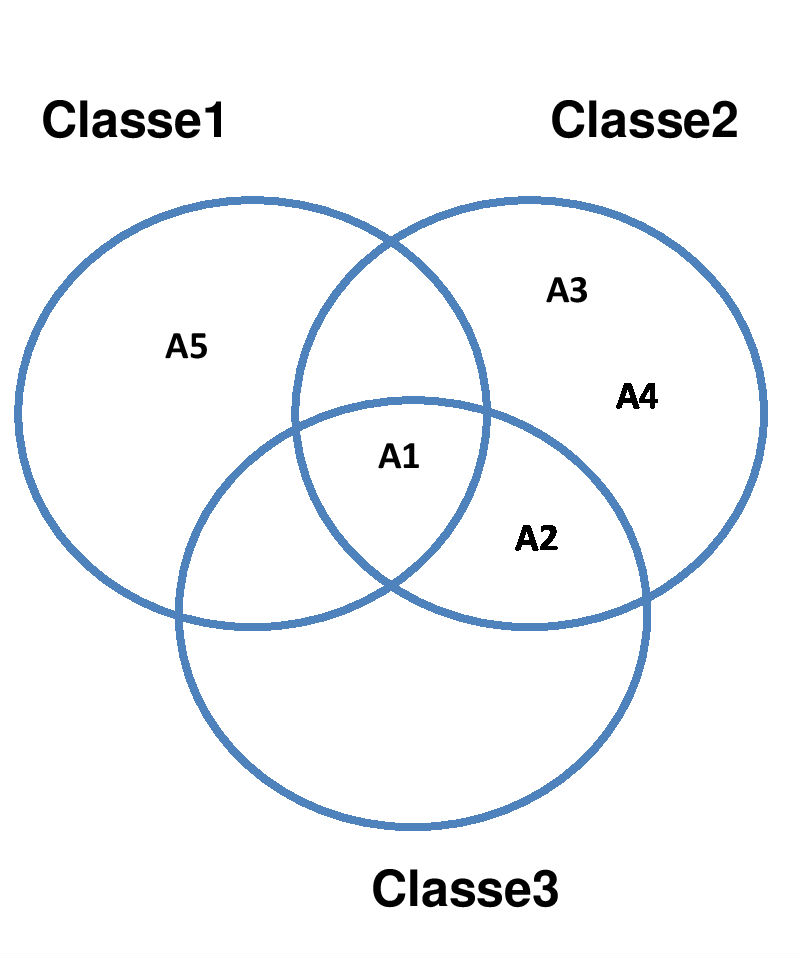
\includegraphics[scale=0.2]{img/classes.jpg}
\caption{classification des attaquants}
\end{figure}
\paragraph{}
Pour classer les attaquants de 1 jusqu'à 5 on va passer par deux étapes basant sur une relation d'ordre dénoté par $\succ$.\newline

\textbf{étape 1:}\newline
dans cet étape on a classé les groupes d'attaquants par rapport à l'ordre des propriétés de sécurité. Les experts de sécurité des systèmes industriels ont classé les propriétés de sécurité avec cet ordre~\cite{ref9} dont ${\succ}_{P}$ représente la priorité de la satisfiabilité des propriétés.
\begin{center}
\textit{Disponibilit\'{e} ${\succ}_{P}$ Int\'{e}grit\'{e} ${\succ}_{P}$ Confidentialit\'{e}}
\end{center}
Dans ce cas et à partir de cet ordre on a classé les 3 classes comme suit, utilisant la relation d'ordre ${\succ}_{C}$ qui répresente la séverité des attaquants de chaque classe.
\[Classe 1\, {\succ}_{C}\, Classe 2\, {\succ}_{C}\, Classe 3\]
Cet ordre signifie que les attaquants de classe1 sont les plus puissants aprés viennent les attaquants de classe2, pour la classe 3 on va pas la considérer car qu'elle regroupe les attaquants de classe 1 et 2.\newline
  
\textbf{étape 2:}\newline
Dans la deuxième étape on doit classer les attaquants de chaque classe à l'aide de nombre des actions de chaque attaquant et le nombre des propriétés qui sont violé par l'attaquant. 
\medskip

\textit{Une action} représente une connaissance de l'attaquant (chiffrer,déchiffrer,...etc).

\begin{table}[!h]
\centering
\begin{tabular}{c|c|c|}
\cline{2-3}
&Nb de propriétés  &Nb d'actions  \\ \hline
\multicolumn{1}{|c|}{$a_1$} &3  & 8 \\ \hline
\multicolumn{1}{|c|}{$a_5$} &1  & 3 \\ \hline
\end{tabular}
\end{table}
\caption{Classification des attaquants de classe 1}
\medskip

Ce tableau nous permet de classifier les attaquants de classe 1 suivant la relation d'ordre ${\succ}_{A}$ qui exprime l'ordre de puissance entre les attaquants. 
\[a_1\; {\succ}_{A}\; a_5\]
\begin{table}[!h]
\centering
\begin{tabular}{c|c|c|}
\cline{2-3}
&Nb de propriétés  &Nb d'actions  \\ \hline
\multicolumn{1}{|c|}{$a_2$} &2  & 5 \\ \hline
\multicolumn{1}{|c|}{$a_3$} &1  & 4 \\ \hline
\multicolumn{1}{|c|}{$a_4$} &1  & 3 \\ \hline
\end{tabular}
\end{table}
\caption{Classification des attaquants de classe 2}
\medskip

À partir de \textit{Table 19} nous permet de classifier les attaquants de classe 2 selon l'ordre suivant:
\[a_2 {\succ}_{A} a_3 {\succ}_{A} a_4\]

à la fin on peut classer les cinq attaquants avec cet ordre :

\newtheorem{Propriete}{Propriété}
\begin{Propriete}
Pour l'ensemble des attaquants $A=\{a_1,\cdots,a_5\}$, on a :
$a_1\, {\succ}_{A}\, a_5\, {\succ}_{A}\, a_2\, {\succ}_{A}\, a_3 {\succ}_{A}\, a_4$.
\end{Propriete}


\subsection{Comparaison entre SPi-calculus et les clauses de Horn}
Le SPi-calculus est suffisamment riche pour modéliser les différents modèles d'attaquant par rapport à les clauses de Horn. On peut voir la différence entre les clauses d'Horn et SPi-calcul dans les points suivants :\newline

\begin{itemize}
\item La représentation de l’attaquant avec les clauses de Horn est basé sur un ensemble des prédicats, par contre avec SPi-calculus l’attaquant est représenté comme un processus.
\item Il existe un ensemble des commandes SPi-calculus comme : \textit{commande parallèle},    \textit{commande alternative}, \textit{commande répétitive},etc.
\item SPi-calculus intègre un mécanisme de synchronisation, par contre pour les clauses de Horn il faut modéliser des prédicats qui expriment l'envoi ou la réception du message.
\item Avec les clauses de Horn il faut définir des prédicats pour exprimer les primitives cryptographiques, par contre à SPi-calculus elles sont déja définies.
\end{itemize}
\newpage
\section{Modèles d'attaquant avec UPPAAL}
UPPAAl~\cite{ref4} est une bo\^{i}te à outils a été développé conjointement par l'université d'Aalborg et l'université d'Uppsala. Il permet de vérifier des réseaux d'automates temporisés. Les propriétés qui peuvent \^{e}tre vérifiées sont principalement des propriétés d'accessibilité, de sûreté, de vivacité ou d'états bloquants. La logique utilisée par UPPAAL est un fragment de TCTL qui n'autorise pas les embo\^{i}tements d'opérateurs temporels. L'algorithme implémenté dans UPPAAL est un algorithme d'analyse en avant.
   
\subsection{Le modèle UPPAAL}
Le modèle qui peut-\^{e}tre vérifié par UPPAAL est une variante des automates temporisés. Ce modèle permet de représenter des contraintes d'urgence (une transition doit \^{e}tre prise immédiatement), des contraintes d'atomicité (une séquence de transitions doit \^{e}tre franchie instantanément). Un automate temporisé est défini comme suit~\cite{ref5} :
\paragraph{Définition :}
Un automate temporisé $A$ est un tuple $\langle N, l_{0}, C, E, I, \Sigma \rangle$ o\`{u} :
\begin{itemize}
\item $N$ est un ensemble fini d'états,
\item $l_{0} \in N$ est l'état initiale,
\item $C$ un ensemble fini d'horloges,
\item $B(C)$ invariant, 
\item $E \subseteq N \times B(C) \times \Sigma \times 2^c \times N$ est un ensemble fini de transitions, 
\item $I : N \longrightarrow B(c)$ associe un invariant à chaque état,
\item $\Sigma$ est un alphabet d'action.\newline
\end{itemize}

Un état de l'automate peut comporter une condition sur les horloges $B(c)$, appelés $invariant$, qui doit \^{e}tre satisfaite pour passer vers l'état suivant. Une transition de l'automate est étiquetée par:
\begin{itemize}
\item une $garde$, qui exprime une condition sur les valeurs des variables, elle doit \^{e}tre satisfaite pour franchir la transition.
\item une $synchronisation$ de la forme $c!$ pour l'émission de signal ou $c?$ pour la réception de signal.
\item une remise à zéro pour certaines horloges et une mise à jour de certaines variables.
\end{itemize}

\subsection{La modélisation de différents modèles d'attaquant}
Les primitives cryptographiques sont représentées par un automate $SecureData$, qui permet de chiffrer, déchiffrer, signer ou vérifier la signature. La figure ci-dessous, représente l'automate $SecureData$ :
\begin{figure}[!h]
\begin{center}
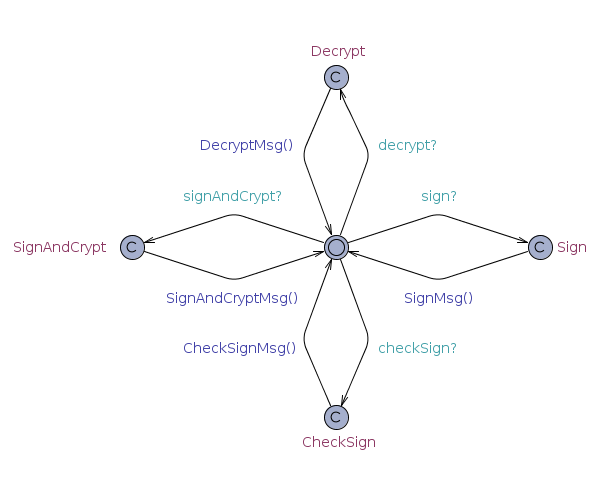
\includegraphics[scale=0.3]{img/secureData.png}\newline
\caption{Automate SecureData.}
\end{center}
\end{figure}

Pour chiffrer un message, on doit calculer $m+2p$ , $m$ est le message et $p$ représente la clé publique. Le déchiffrement s'effectue avec $m-s$ , $s$ représente la clé privée et $s=2p$. Les agents de réseaux peuvent utiliser cet automate à l'aide des canaux de communication $sign$, $signAndCrypt$, $decrypt$ et $checkSign$.
\subsubsection{Attaquant 1 :}
La figure 3 représente un attaquant qui fonctionne comme \textit{Dolev-Yao}. Il peut recevoir et envoyer les messages à travers le canal $c2s$. La variable locale $i$ borne le nombre total d'actions autorisées à faire à chaque tour. Si l'attaquant déplace à l'état $I1$, il peut décider de faire les actions :
\begin{itemize}
\item sélectionner une clé publique (état $I3$).
\item sélectionner une clé privée (état $I5$).
\item copier un message(état $I6$).
\item rejouer un message(état $I7$).
\item forger un message(état $8$).
\item chiffrer, signer et chiffrer ou déchiffrer un message(état $I10$).
\item modifier une partie de message(état $I11$).
\end{itemize}
De plus, l'attaquant peut continuer à faire ces actions, choisir d'envoyer un message ou de bloquer un message.        
\begin{figure}[!h]
\centering 
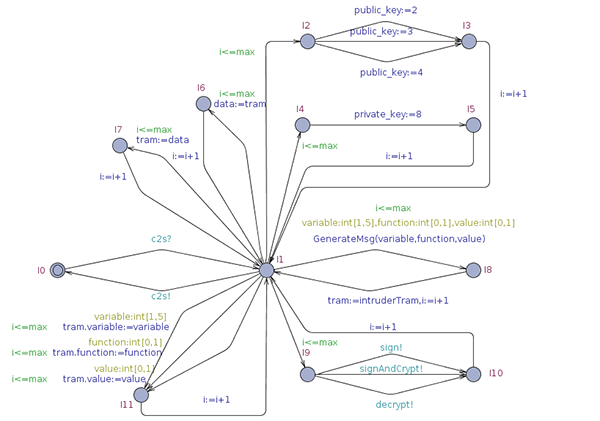
\includegraphics[scale=0.5]{img/attaquant1-600.png}
\caption{Automate de l'attaquant 1.}
\end{figure}

\subsubsection{Attaquant 2 :}
Le rôle principal de cet attaquant est de modifier une partie du message ou le message complet à partir de ses connaissances. Si l'attaquant déplace à l'état $I1$, il peut décider de faire les actions :
\begin{itemize}
\item sélectionner une clé publique (état $I3$).
\item sélectionner une clé privée (état $I5$).
\item chiffrer, signer et chiffrer ou déchiffrer un message (état $I8$).
\item modifier une partie de message (état $I6$).\newpage
\end{itemize}
\begin{figure}[!h]
\centering 
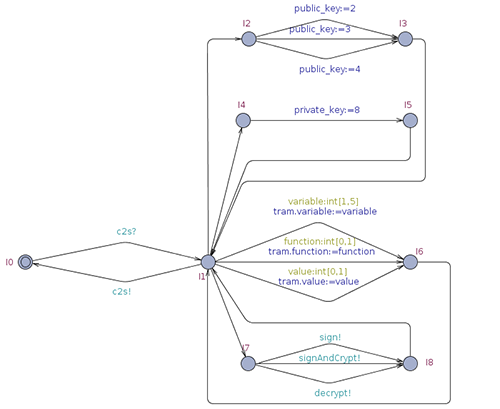
\includegraphics[scale=0.5]{img/attaquant2-500.png}
\caption{Automate de l'attaquant 2.}
\end{figure}
\subsubsection{Attaquant 3 :}
Le rôle principal de cet attaquant est de forger les messages par la technique force brute à partir de ses connaissances. Si l'attaquant déplace à l'état $I1$, il peut décider de faire les actions :  
\begin{itemize}
\item sélectionner une clé publique (état $I3$).
\item sélectionner une clé privée (état $I5$).
\item chiffrer, signer et chiffrer ou déchiffrer un message (état $I8$).
\item forger un message message (état $I6$).
\end{itemize}

\begin{figure}[!h]
\centering 
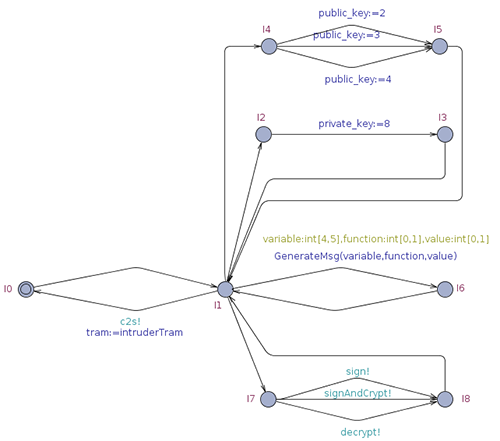
\includegraphics[scale=0.5]{img/attaquant3-500.png}
\caption{Automate de l'attaquant 3.}
\end{figure}

\subsubsection{Attaquant 4 :}
Le rôle principal de cet attaquant est de rejouer les messages. Pour rejouer les messages l'attaquant d'abord se deplace vers l'état $I1$ pour copier le message dans la variable $data$ et après se deplacer vers l'état $I2$ pour rejouer le message. La figure ci-dessous, représente l'automate de l'attaquant 4:  

\begin{figure}[!h]
\centering 
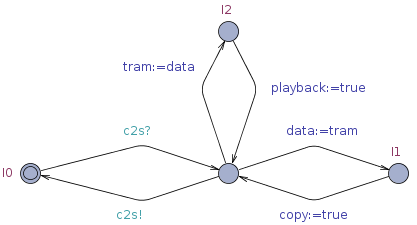
\includegraphics[scale=0.5]{img/attaquant4.png}
\caption{Automate de l'attaquant 4.}
\end{figure}

\subsubsection{Attaquant 5 :}
Le rôle principal de cet attaquant est de bloquer ou retarder les messages. L'attaquant dans l'état $I1$ peut décider de retourner vers l'état $I0$ sans envoyé le message. Dans ce cas, le message sera bloque ou envoy\'e après une periode du temps, c’est-à-dire dans ce cas le message arrivera en retard. La figure ci-dessous, représente l'automate de l'attaquant 5.  

\begin{figure}[!h]
\centering 
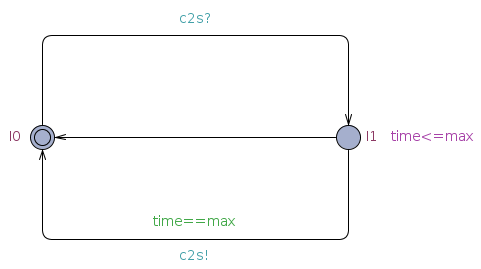
\includegraphics[scale=0.4]{img/attaquant5.png}
\caption{Automate de l'attaquant 5.}
\end{figure}

\section{Conclusion}
Dans ce rapport on a présenté les différents modèles d'attaquant et leurs modélisations avec le model checking UPPAAL. Cependant, au vu des résultats obtenus lors de la mise en pratique, il appara\^{i}t que ce modèle peut trouver des attaques dans un temps raisonnable.\newline

Dans le travail futur on veut utiliser les modèles d'attaquant probabiliste pour contr\^{o}ler l'indéterminisme des attaquants pour reduire l'espace d'état du model checking.  



\newpage
\bibliography{mabiblio}
\bibliographystyle{plain}

\end{document}
